\documentclass[12pt, a4paper]{article}

\usepackage{setspace}
\usepackage[utf8]{inputenc}
\usepackage[legalpaper, margin=1in]{geometry}
\usepackage{siunitx}
\usepackage{amsmath,amsthm,mathtools}
\usepackage{amsfonts} 
\usepackage{systeme}
\usepackage{hyperref}
\usepackage{graphicx}
\usepackage{listings}
\usepackage{xcolor}
\usepackage{float}

\definecolor{codegreen}{rgb}{0,0.6,0}
\definecolor{codegray}{rgb}{0.5,0.5,0.5}
\definecolor{codepurple}{rgb}{0.58,0,0.82}
\definecolor{backcolour}{rgb}{0.95,0.95,0.92}

\lstdefinestyle{mystyle}{
    backgroundcolor=\color{backcolour},   
    commentstyle=\color{codegreen},
    keywordstyle=\color{magenta},
    numberstyle=\tiny\color{codegray},
    stringstyle=\color{codepurple},
    basicstyle=\ttfamily\footnotesize,
    breakatwhitespace=false,         
    breaklines=true,                 
    captionpos=b,                    
    keepspaces=true,                 
    numbers=left,                    
    numbersep=5pt,                  
    showspaces=false,                
    showstringspaces=false,
    showtabs=false,                  
    tabsize=2
}

\lstset{style=mystyle}


\title{Differential Equations \\ Computational Practicum 1 \\ Variant 2}
\author{Rizvan Iskaliev \\ r.iskaliev@innopolis.university \\ Innopolis University, BS19-04}
\date{29 October 2020}

\begin{document}
\maketitle

\section{Analytical solution}
    \begin{center}
         We are given the equation: \\
         $y' = \frac{y}{x} - xe^{\frac{y}{x}}$
    \end{center}
    
    \begin{itemize} 
        \item We have $\frac{y}{x}$ and $e^{\frac{y}{x}}$ terms in which $x$ is in denominator.
        \item $x = 0$ - point of discontinuity (infinite discontinuity)
        \item Let $\frac{y}{x} = t$. Then $y = tx$ and $y' = t'x + t$. Let us substitute it into original equation:
    \end{itemize}
    
    \begin{center}
         $t'x + t = t - xe^{t} \Leftrightarrow t'x = -xe^{t} \Leftrightarrow \frac{dt}{dx} = -e^{t} \Leftrightarrow dt = -e^{t}dx$ \\
         Since $e^{t} \neq 0$ for $t \in \mathbb{R}$ then let us divide both sides of the equation by $-e^{t}$: \\
         $-\frac{dt}{e^{t}} = dx$ \\
    \end{center}
    
    \begin{itemize}
        \item Let us integrate both sides of the equation:
    \end{itemize}
    \begin{center}
        $-\int_{}^{}\frac{dt}{e^{t}} = \int_{}^{}dx$ \\
        $e^{-t} = x + C$, where $C$ is some real constant \\
        From this $C = e^{-t} - x = e^{-\frac{y}{x}} - x$ \\
    \end{center}
    
    \begin{itemize}
        \item Let us take the logarithm of both sides of the equation:
    \end{itemize}
    
    \begin{center}
        $ln(e^{-t}) = ln(x + C) \Leftrightarrow -t = ln(x + C) \Leftrightarrow t = -ln(x + C)$\\
        By the properties of logarithm, $x + C > 0 \Leftrightarrow x + e^{-\frac{y}{x}} - x > 0 \Leftrightarrow e^{-\frac{y}{x}} > 0$ \\
        And this holds for $x \in \mathbb{R} \setminus \{0\}$
    \end{center}
    
    \begin{itemize}
        \item Let us substitute $\frac{y}{x}$ back into $t$:
    \end{itemize}
    
    \begin{center}
        $\frac{y}{x} = -ln(x + C) \Leftrightarrow y = -x \cdot ln(x + C)$ \\
        Thus, $y = -x \cdot ln(x + C)$, where $C$ is some real constant, is the general solution of the $y' = \frac{y}{x} - xe^{\frac{y}{x}}$ on $x \in (-\infty; 0) \cup (0; +\infty)$ \\
    \end{center}
    
    \begin{itemize}
        \item Let us solve the initial value problem: we have that $y(1) = 0$ 
    \end{itemize}
    
    \begin{center}
        By substituting the corresponding values of $x$ and $y$, we obtain that $C = e^{0} - 1 = 1 - 1 = 0$ and $y = -x \cdot lnx$ is the solution of I. V. P. \\
    \end{center}
\newpage
\section{Programming part}

    In this work I programmed on Python 3.8.\\ GitHub repository of this project: \url{https://github.com/rizvansky/DE-Assignment-1} 
    \subsection{Packages}
        \begin{enumerate}
            \item \textbf{PyQt5} (implement GUI (Graphical User Interface))
            \item \textbf{numpy} (calculations and operations with arrays)
            \item \textbf{sys} (setup the interpreter and run the application correctly)
            \item \textbf{matplotlib} (plot the graphs and navigate over them)
        \end{enumerate}
        
    \subsection{GUI implementation}
    My program work as follows: \\ When pressing \textbf{Plot solutions} button, the method to plot graphs is called. If input values are valid, graphs of solutions, local errors and max GTE with respect to N are plotted on corresponding tabs. Otherwise, the message box(es) will appear with corresponding error text. Also, below the part where user can specify input parameters, an application has checkboxes for showing / hiding metrics of particular solution methods. Each of checkboxes is connected with function that shows / hides plots that user specifies. See an $interesting$ part of a code for GUI implementation below: 
    \\

    \begin{lstlisting}[language=Python, caption=\_\_init\_\_ method of ApplicationWindow class (Main window of GUI). GraphsTabWidget and OptionsWidget are composite widgets (also classes) for graphs and options setting correspondingly.]
from PyQt5 import QtWidgets
from helper_widgets import GraphsTabWidget, OptionsWidget
import numpy as np
from methods import EulerMethod, ImprovedEulerMethod, RungeKuttaMethod
    

class ApplicationWindow(QtWidgets.QMainWindow):
    def __init__(self, euler, improvedEuler, rungeKutta):
        super(ApplicationWindow, self).__init__()

        self.euler = euler
        self.improvedEuler = improvedEuler
        self.rungeKutta = rungeKutta

        self.graphsTabWidget = GraphsTabWidget(self)

        self.optionsWidget = OptionsWidget(self)
        self.optionsWidget.plotButton.clicked.connect(self.plotGraphs)
        self.optionsWidget.methodsCheckboxesWidget.checkboxExact.stateChanged.connect(self.plotGraphs)
        self.optionsWidget.methodsCheckboxesWidget.checkboxEuler.stateChanged.connect(self.plotGraphs)
        self.optionsWidget.methodsCheckboxesWidget.checkboxImprovedEuler.stateChanged.connect(self.plotGraphs)
        self.optionsWidget.methodsCheckboxesWidget.checkboxRungeKutta.stateChanged.connect(self.plotGraphs)

        self.mainLayout = QtWidgets.QHBoxLayout()
        self.mainLayout.addWidget(self.graphsTabWidget)
        self.mainLayout.addWidget(self.optionsWidget)
        self.mainWidget = QtWidgets.QWidget()
        self.mainWidget.setLayout(self.mainLayout)
        self.setCentralWidget(self.mainWidget)

        self.setWindowTitle('DE solver')

        self.plotGraphs()
    \end{lstlisting}
    
    \newpage
    \begin{lstlisting}[language=Python, caption=plotGraphs method of ApplicationWindow class]
def plotGraphs(self):
    params = self.getParameters()

    if params is not None:
        self.graphsTabWidget.solutionsGraphs.clear()
        self.graphsTabWidget.gteGraphs.clear()
        self.graphsTabWidget.gteMaxGraphs.clear()

        axes = {
            'solutions': self.graphsTabWidget.solutionsGraphs.add_subplot(111),
            'gte': self.graphsTabWidget.gteGraphs.add_subplot(111),
            'gteMax': self.graphsTabWidget.gteMaxGraphs.add_subplot(111)
        }

        self.updateSolutions(params['x0'], params['y0'], params['X'], params['N'])
        gteMaxEuler, gteMaxImprovedEuler, gteMaxRungeKutta, nPoints = self.calculateGteMax(params['x0'], params['y0'],
                                                                                            params['X'], params['n0'],
                                                                                            params['nMax'])

        xPoints = self.euler.xPoints
        if self.optionsWidget.methodsCheckboxesWidget.checkboxExact.isChecked():
            self.setGraph(axes, xPoints, self.euler.yExactValues, np.zeros(shape=[len(self.euler.xPoints)]),
                        np.zeros(shape=[len(nPoints)]), nPoints, 'c', 'Exact')

        if self.optionsWidget.methodsCheckboxesWidget.checkboxEuler.isChecked():
            self.setGraph(axes, xPoints, self.euler.yApproxValues, self.euler.gte, gteMaxEuler, nPoints, 'b',
                        'Euler')

        if self.optionsWidget.methodsCheckboxesWidget.checkboxImprovedEuler.isChecked():
            self.setGraph(axes, xPoints, self.improvedEuler.yApproxValues, self.improvedEuler.gte,
                              gteMaxImprovedEuler, nPoints, 'r', 'Improved Euler')

        if self.optionsWidget.methodsCheckboxesWidget.checkboxRungeKutta.isChecked():
            self.setGraph(axes, xPoints, self.rungeKutta.yApproxValues, self.rungeKutta.gte,
                              gteMaxRungeKutta, nPoints, 'm', 'Runge-Kutta')

        self.graphsTabWidget.solutionsCanvas.draw()
        self.graphsTabWidget.gteCanvas.draw()
        self.graphsTabWidget.gteMaxCanvas.draw()
    \end{lstlisting}
    
    \subsection{Solution methods implementation}
        \textbf{DifferentialEquation} is the class that consists of the following fields: $f$ and $exactSolution$ - these are the expressions of $f(x, y)$ and exact solution correspondingly. \\
        \textbf{SolutionMethod} is the parent class for \textbf{EulerMethod}, \textbf{ImprovedEulerMethod} and \textbf{RungeKuttaMethod} classes. \textbf{SolutionMethod} contains fields for: approximated and exact $y$ values, $x$ values, step size, local errors, source differential equation and methods for: calculating the exact solution, $x$ values needed for approximation and local errors. Classes that are inherited from this class (approximation methods) have the same fields as the parent class but have new methods for approximating the solution and calculating local errors. For example, see the code for SolutionMethod (parent class) and RungeKuttaMethod (child class):
        
        \begin{lstlisting}[language=Python, caption=DifferentialEquation class]
class DifferentialEquation:
    def __init__(self, f, exactSolution):
        self.f = f
        self.exactSolution = exactSolution
    \end{lstlisting}
        
        \begin{lstlisting}[language=Python, caption=SolutionMethod class]
import numpy as np


class SolutionMethod:
    def __init__(self, diffEquation):
        self.diffEquation = diffEquation
        self.h = 0
        self.xPoints = np.array([])
        self.yExactValues = np.array([])
        self.yApproxValues = np.array([])
        self.gte = np.array([])

    def setXPoints(self, x0, X, N):
        self.xPoints = np.array([x0])

        self.h = (X - x0) / N
        for i in range(1, N):
            self.xPoints = np.append(self.xPoints, x0 + self.h * i)

    def calculateYExactValues(self, x0, y0, N):
        self.yExactValues = np.array([y0])

        C = np.exp(-y0 / x0) - x0

        for i in range(1, N):
            self.yExactValues = np.append(self.yExactValues, self.diffEquation.exactSolution(self.xPoints[i], C))

    def calculateGTE(self, N):
        self.gte = np.array([0])

        for i in range(1, N):
            self.gte = np.append(self.gte, np.abs(self.yExactValues[i] - self.yApproxValues[i]))
    \end{lstlisting}
    
    \begin{lstlisting}[language=Python, caption=RungeKuttaMethod class]
class RungeKuttaMethod(SolutionMethod):
    def __init__(self, diffEquation):
        SolutionMethod.__init__(self, diffEquation)

    def k1(self, i):
        return self.diffEquation.f(self.xPoints[i], self.yApproxValues[i])

    def k2(self, i):
        return self.diffEquation.f(self.xPoints[i] + self.h / 2, self.yApproxValues[i] + self.h / 2 * self.k1(i))

    def k3(self, i):
        return self.diffEquation.f(self.xPoints[i] + self.h / 2, self.yApproxValues[i] + self.h / 2 * self.k2(i))

    def k4(self, i):
        return self.diffEquation.f(self.xPoints[i] + self.h, self.yApproxValues[i] + self.h * self.k3(i))

    def solve(self, x0, y0, X, N):
        self.h = (X - x0) / N
        self.setXPoints(x0, X, N)
        self.calculateYExactValues(x0, y0, N)
        self.calculateYApproxValues(y0, N, self.h)
        self.calculateGTE(N)

    def calculateYApproxValues(self, y0, N, h):
        self.yApproxValues = np.array([y0])

        for i in range(N - 1):
            self.yApproxValues = np.append(self.yApproxValues, self.yApproxValues[i] + h / 6 * (self.k1(i) +
                                                                    2 * self.k2(i) + 2 * self.k3(i) + self.k4(i)))
    \end{lstlisting}
    
\section{UML diagram}
UML diagram was created using built-in PyCharm IDE tool for automatic UML diagram creation.
    \begin{figure}[H]
        \centering
        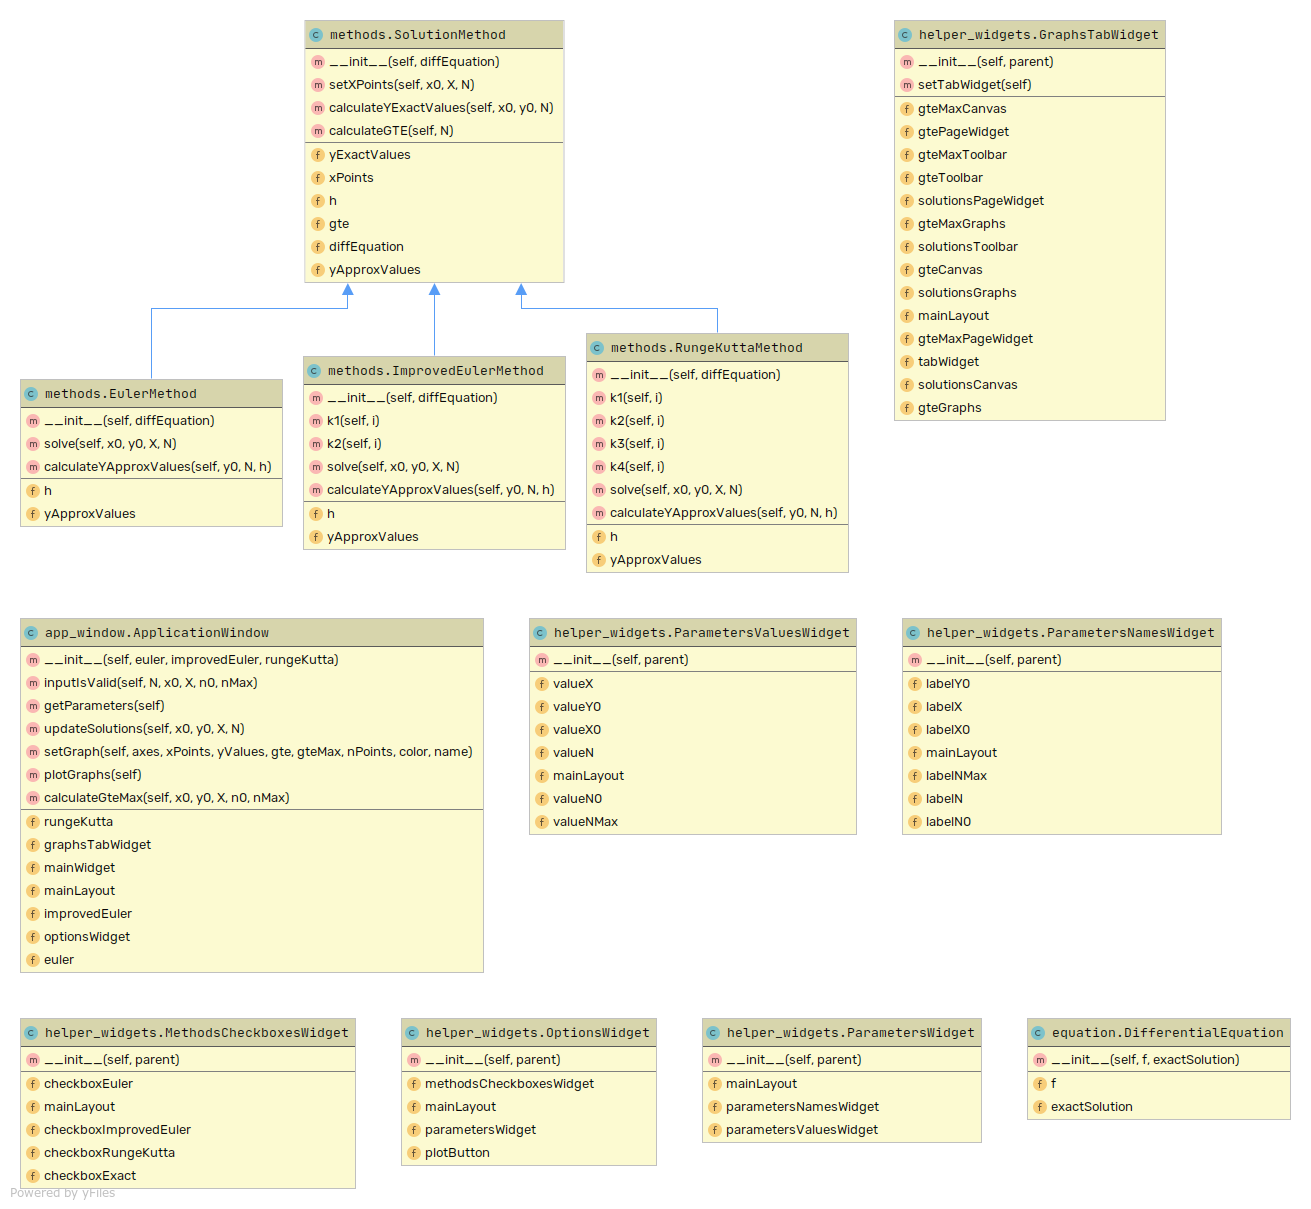
\includegraphics[scale=0.4]{uml}
        \caption{UML diagram}
        \label{fig:my_label}
    \end{figure}

\newpage
\section{GUI and graphs plotting}
Below are the graphs for exact solution and solutions obtained by approximation methods with parameters that are specified in statement of my variant:
\begin{itemize}
    \item Differential Equation: $y' = \frac{y}{x} - xe^{\frac{y}{x}}$
    \item $x_0 = 1$
    \item $y_0 = 0$
    \item $X = 8$
\end{itemize}

I choose $N = 30$ and selected the interval for $N$ for convergence analysis to be $[10; 100]$ \\
These parameters can be changed in application window and new graphs will be plotted. 

\begin{figure}[H]
        \centering
        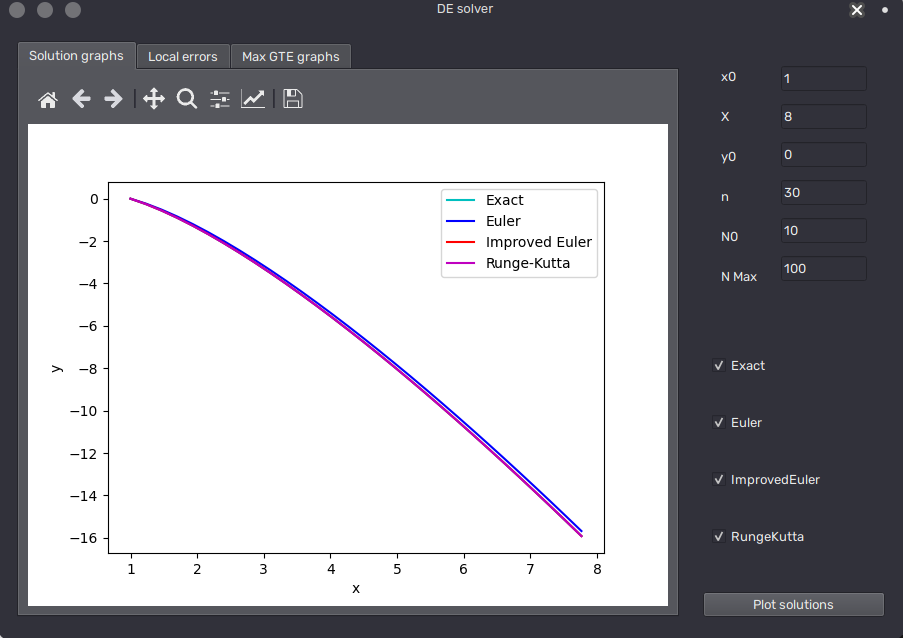
\includegraphics[scale=0.6]{gui_solutions}
        \caption{Solutions}
        \label{fig:my_label}
    \end{figure}
    
    \begin{figure}[H]
        \centering
        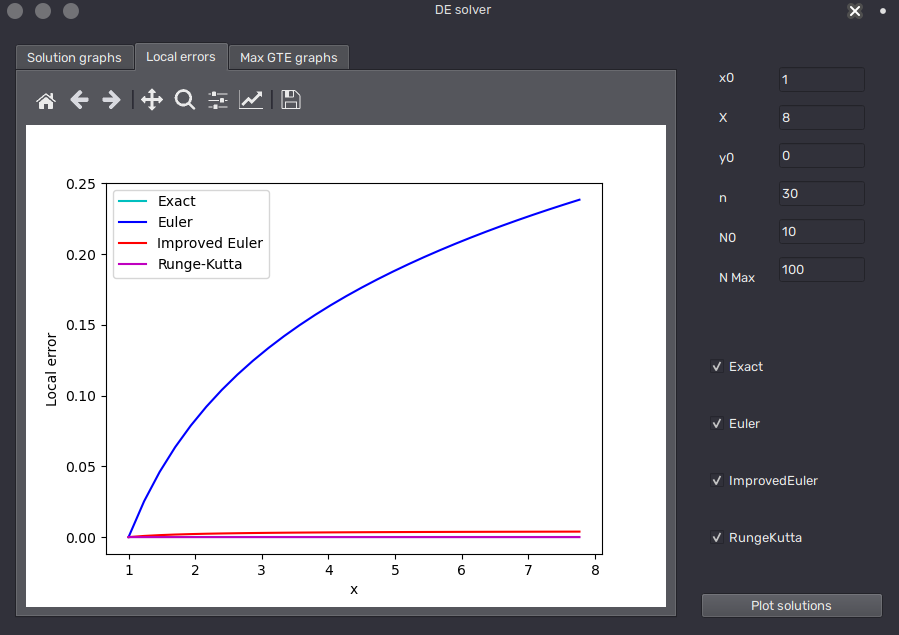
\includegraphics[scale=0.6]{gui_lte}
        \caption{Local errors}
        \label{fig:my_label}
    \end{figure}
    
    \begin{figure}[H]
        \centering
        \includegraphics[scale=0.6]{gui_gte_max}
        \caption{Approximation errors of these methods for different grid sizes}
        \label{fig:my_label}
    \end{figure}

\begin{center}
We see that from the listed approximation methods, local error of Runge-Kutta method is the smallest one. Then goes Improved Euler's method. And the method with the largest local error is Euler's method. 

From the third graph we conclude that the approximation error decreases with increasing of $N$. \\
And if $N$ tends to $+\infty$ then local error tends to 0.
\end{center}

\end{document}